\documentclass{report}
\usepackage[utf8]{inputenc}
\usepackage[spanish]{babel}
\usepackage[letterpaper, portrait, margin=2cm]{geometry}
\usepackage[style=ieee]{biblatex}
\usepackage{amsthm}
\usepackage{amsmath}
\usepackage{amssymb}
\usepackage{amsfonts}
\usepackage{hyperref}
\usepackage{csquotes}
\usepackage{mathtools}
\usepackage{graphicx}
\usepackage{float}
\usepackage{array}
\usepackage{dirtytalk}
\usepackage[table,xcdraw]{xcolor}

\addbibresource{bibliography.bib}

\newtheorem{definition}{Definición}

\DeclarePairedDelimiter{\ceil}{\lceil}{\rceil}

\title{Marco Teórico de Investigación: Modelo de muestreo virtual de suelos agrícolas en Honduras para analítica en base al muestreo aleatorio simple y estratificado}
\author{Tobias Briones \bigbreak tobias.briones@unah.hn}
\date{Noviembre 2021}

\begin{document}

\makeatletter
    \begin{titlepage}
        \begin{center}
            
\includegraphics[width=0.3\linewidth]{ref/logo-unah.png}\\[4ex]
            {\huge \bfseries \@title 
            \vspace{1cm}}\\[2ex]
            {\LARGE \@author}\\[50ex] 
            
            {\large
            Anteproyecto de seminario de investigación presentado a la\\
            Universidad Nacional Autónoma de Honduras de la carrera de\\
            Licenciatura en Matemática
            }\\[2ex]
            
            {\large \@date}
        \end{center}
    \end{titlepage}
\makeatother
\thispagestyle{empty}
\newpage

\thispagestyle{empty}
\tableofcontents
\listoffigures
\newpage

\chapter{Marco teórico}

El muestreo surge de la necesidad de reducir la cantidad de candidatos que van a ser sometidos a un análisis estadístico siempre que estos representen al total de la población en la que pertenecen, es decir, que se obtengan resultados muy similares al hacer el estudio bajo esa muestra como si si hicieran con toda la población. El problema claramente es que las poblaciones (total de individuos de interés para dicho estudio) son a menudo demasiado grandes. Un buen muestreo permite no tener que estudiar a todos los elementos de una población. 

\bigbreak

Como ejemplificación, tenemos que en este estudio, la entrada del sistema es un conjunto de datos del usuario que es ya un muestreo realizado previamente por este. Como se sabe, en la profesión de la ciencia de datos, una de las etapas primeras es obtener e identificar los datos útiles previo al análisis \cite{university-of-wisconsin-data-science-2021}. Los modelos que se deben entrenar llevan una sobrecarga en el tamaño de las entradas que se obtienen por lo que con la definición de muestra dada arriba, se tiene que, se ha de obtener una muestra de los \say{datos sucios} proveídos por el usuario a fin de conseguir una carga menor para los modelos de analítica y produciendo los mismos resultados, esto es, minimizar los datos de entrada de los modelos de ciencia de datos para estudios agrícolas, tema que apunta directamente al objetivo principal de este estudio.

\bigbreak

Muestreos buenos ocasionalmente producirán malos resultados y sistemas malos ocasionalmente producirán buenos resultados \cite{gulland-1966}. Por esto, es importante repetir los experimentos para comprender la distribución de frecuencia del sistema el cual deberá dar una varianza pequeña.

\bigbreak

Entre los tipos de muestreo que se han encontrado útiles para medir los suelos agrícolas se tienen:

\begin{itemize}
    \item \textbf{Muestreo Aleatorio Simple (MAS):} Consiste en tomar $n$ puntos aleatorios de la población. Estos puntos deben de tener la misma probabilidad de ser escogidos para que la muestra sea representativa y se toman de forma \say{mezclada}. Por ejemplo, la sangre esta \say{mezclada} en el cuerpo humano, por lo que al tomar una muestra de solo una pizca basta para hacer los análisis ya que esa pizca obtenida es igual que todas las demás.
    
    \item \textbf{Muestreo Simple Estratificado:} Esta es una técnica de muestreo que será muy útil en el modelado de los suelos agrícolas. La población se particiona en subconjuntos de diferentes tipos y homogéneos de forma que se puede realizar un MAS en cada subconjunto homogéneo de la partición. Por ejemplo, los lotes se pueden particionar como: área forestal, con problemas, bosque, construcción, etc.
    
    \item \textbf{Muestreo Sistemático:} En este muestreo se toma un punto aleatorio y se mide por cada $n$-ésima unidad de forma que se lleva un espaciado constante a partir del punto inicial. Por ejemplo, este tipo de muestreo es utilizado para medir el suelo cuando es rectangular a lo largo de su perímetro o también cuando es de forma irregular.
\end{itemize}

\section{Marco para muestreo}

El marco para muestreo \cite{lohr-2009} consiste en definir el espacio de la población (el universo) de donde se obtendrán las posibles muestras (subconjuntos) y estas muestras contienen las unidades que serán seleccionadas. Se nota que cada muestra tiene una probabilidad de ser escogida y para cada muestra, cada unidad tiene también una probabilidad para ser escogida.

\begin{definition}[Universo]
    El \textbf{Universo} o \textbf{Población finita} de $N$ unidades es el conjunto índice
    $$
    U = \{ 1, 2, ..., N \}
    $$
    Donde $N \in \mathbb{N}$ es el tamaño de la población.
\end{definition}

\begin{definition}[Muestra]
    Sea $U$ el conjunto universo. Un conjunto $S$ es una muestra para $U$ si $S \subseteq U$.
\end{definition}

\begin{definition}[Probabilidad de una muestra]
    Si $S$ es una muestra. $S$ tiene una probabilidad de ser escogida de $P(S)$.
\end{definition}

Notar que la probabilidad de todas las muestras de ser escogida es $1$. Esto es, $\forall S_i \in D \implies \sum_{i=1}^{N} P(S_i) = 1$, donde el conjunto $D$ es el diseño escogido, esto es, una colección de subconjuntos (muestras) de $U$.

\bigbreak

Según las definiciones de arriba, cada muestra $S_i$ tiene probabilidad $P(S_i)$ de ser seleccionada. Ahora, cada unidad tiene una probabilidad de terminar siendo seleccionada si pertenece a una de las muestras que se seleccionó.

\begin{definition}[Probabilidad de una Unidad]
    La probabilidad de que una unidad $x$ sea seleccionada en una colección de muestras $D = \{ S_1, S_2, ..., S_n \}$ se define como
    
    $$
    \pi_x = P(\text{unidad $x$ está en la muestra}) = \sum_{S_i \in \{ S \in D | x \in S \}} P(S_i)
    $$
\end{definition}

Es decir, para calcular la probabilidad de que la unidad $x$ sea seleccionada, se hace la suma de las probabilidades de todas las muestras que contienen a $x$.

Con respecto a los intervalos de confianza, se deberá repetir muchas veces el muestreo para por determinar su confianza. Son útiles en el caso no-ideal donde no se conoce toda la población. Los intervalos de confianza se construyen como \cite{the-pennsylvania-state-university-no-date}:

\begin{definition}[Intervalo de confianza]
    Un \textbf{intervalo de confianza} es un rango que se calcula usando estadística para estimar un parámetro desconocido de la población con un nivel determinado de confianza. 
\end{definition}

\begin{definition}[Sesgo de una muestra]
    El \textbf{sesgo de una muestra} es la diferencia de la media estimada y el valor real.
\end{definition}

\begin{definition}[Estimación puntual]
    La \textbf{estimación puntual} es una muestra estadística que sirve como los mejores estimados para un parámetro de la población.
\end{definition}

\begin{definition}[Margen de error]
    El \textbf{margen de error} de un intervalo de confianza es la mitad de su ancho.
\end{definition}

\begin{definition}[Diseño muestral]
    Un \textbf{diseño muestral} es una función $p(X)$ que asigna una probabilidad de selección a cada posible muestra en el espacio muestral $\omega$.
    
    \bigbreak
    
    Sea $S^* = \mathcal{P}(U)$ el conjunto potencia de $U$, esto es, el conjunto de todas las posibles muestras de la población $U$. Un diseño muestral es \textbf{sin reemplazo} si todas las muestras en $S^*$ son sin reemplazo. Análogamente, es un muestreo \textbf{con reemplazo} si todas las muestras en $S^*$ son con reemplazo.

    \bigbreak
    
    En una \textbf{muestra aleatoria sin reemplazo} la selección de los elementos que han sido seleccionados no vuelven a ser parte de la población. En una \textbf{muestra aleatoria con reemplazo} la selección de de los elementos que han sido seleccionados vuelven a ser parte de la población, es decir, un elemento puede ser seleccionado más de una vez.
\end{definition}

\section{Estimar el tamaño de la muestra}

Al estimar el tamaño de la muestra se tiene en cuenta otras definiciones como el margen de error que se considera tolerable. Las encuestas se pueden llevar a cabo para obtener estas condiciones correctamente. Para obtener resultados con respecto al tamaño de muestra preferible se sugiere \cite{lohr-2009}:

\begin{enumerate}
    \item Preguntárse: ¿Qué se espera de la muestra, y cuánta precisión se necesita?, ¿Qué consecuencias tienen los resultados del muestreo?, ¿Cuánto error es tolerable?.
    
    \item Encontrar una ecuación que relacione el tamaño de la muestra $n$ y las expectativas de la muestra.
    
    \item Estimar cualquier cantidad desconocida y resolver para $n$.
    
    \item Iterar estos pasos para obtener mejores valores de acuerdo a las expectativas. Si ni siquiera hay recursos disponibles para este proceso, entonces la investigación no se podrá llevar a cabo.
\end{enumerate}

\section{Muestreo aleatorio simple (MAS)}

Este tipo de muestreo es el más básico que se puede tomar y en base a él se desarrollan en gran medida los otros tipos de muestreo más compuestos. Las condiciones para que funciones son que las unidades de la población tenga igual probabilidad de ser escogidas. Los cálculos hechos para el MAS son también extendidos por otros métodos de muestreo, ya que al final siempre conllevan con algo de aleatoriedad. 

\bigbreak

Es importante que el suelo sea homogéneo para realizar un muestreo simple aleatorio y probablemente también mezclar las muestras para obtener un compuesto. Para realizar el muestreo se pueden seguir varios patrones, a saber, zigzag, diagonal, etc.:

\begin{figure}[H]
    \centering
    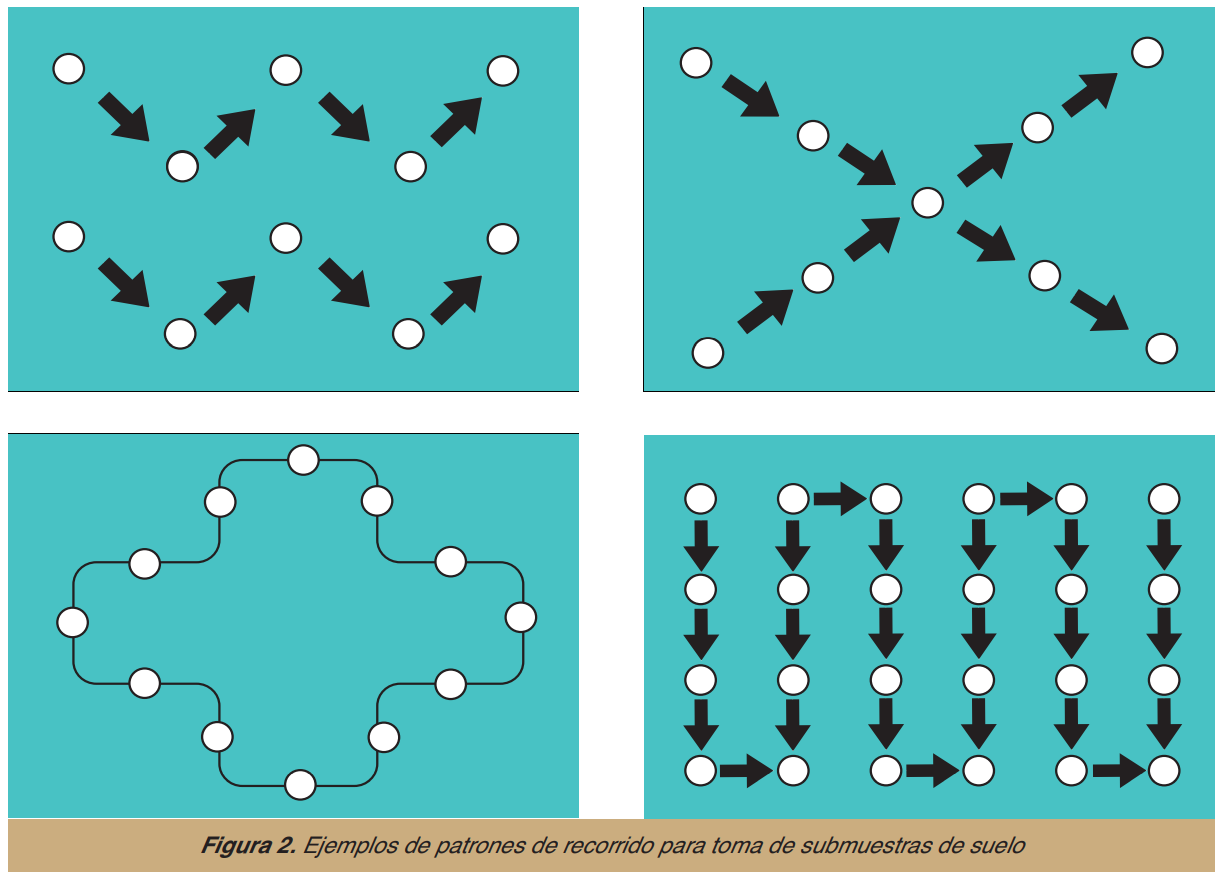
\includegraphics[width=0.3\paperwidth]{ref/sampling-patterns-srs.png}
    \caption{Patrones de muestreo para análisis de fertilidad de suelo \cite{lassaga-2011}}
\end{figure}

Como se detalla más adelante, el terreno o lotes también se puede estratificar y realizar un MAS en cada estrato obtenido. El muestro sistemático por otra parte puede llegar a reducirse a un MAS o similar dado las condiciones apropiadas. Esto indica que el MAS es elemental para hacer otro tipo de diseño de muestreo.

\bigbreak

Estas son los resultados para los cálculos del MAS \cite{thompson-2012}:

\bigbreak
\textbf{Media de la población}

\bigbreak

$\overline{x}_U = \frac{1}{N}(x_1 + x_2 + ... + x_N) = \frac{1}{N} \sum_{i=1}^N x_i$


\bigbreak
\textbf{Media de la muestra}

\bigbreak

$\overline{x} = \frac{1}{n}(x_1 + x_2 + ... + x_N) = \frac{1}{n} \sum_{i=1}^n x_i$


\bigbreak
\textbf{Varianza de la población finita} En MAS, la varianza de la muestra $s^2$ es una estimación no-alineada de la varianza para la población finita

\bigbreak

$\sigma ^2 = \frac{1}{N-1} \sum_{i=1}^{N} (x_i - \overline{x}_U)^2$


\bigbreak
\textbf{Varianza de la muestra}

\bigbreak

$s^2 = \frac{1}{n-1} \sum_{i=1}^n (x_i - \overline{x}_U)^2$


\bigbreak
\textbf{Total de la población}

\bigbreak

$t = \sum_{i=1}^N x_i = N \overline{x}_U$


\section{Muestreo sistemático}

Para realizar un muestreo sistemático se siguen los siguientes cálculos:

\bigbreak

Dado el tamaño de la población $N$ y el número de muestras $n$, hacer $k=\ceil{\frac{N}{n}}$. El valor $k$ es el período que hace que el muestreo sea sistemático. Tomar un punto aleatorio $K \in [1, k]$. Cada unidad dada por $K$, $K + k$, $K + 2k$, ... , etc., define la muestra.

\bigbreak

En ciertos casos el muestreo sistemático es el mismo MAS por lo que se pueden aplicar técnicas del MAS. Otras veces funciona como un intermediario (proxy) hacia el MAS ya que como se puede notar, si la población está dispuesta de forma aleatoria entonces lo que se tendría sería básicamente un MAS. También se debe tener en cuenta que la probabilidad de un grupo de ser escogido no es la misma como en el MAS. Otro uso que puede tener este tipo de muestreo es de hacer un trabajo similar al muestreo por clúster. De estos factores depende que la muestra sea representativa ya que si la población está ordenada de acuerdo a su índice entonces la muestra no servirá (p. ej. solo salen unidades del mismo tipo al estar ordenadas por posición, si hay hombres y mujeres solo salen hombres por ser posición par). 

\bigbreak

\begin{figure}[H]
    \centering
    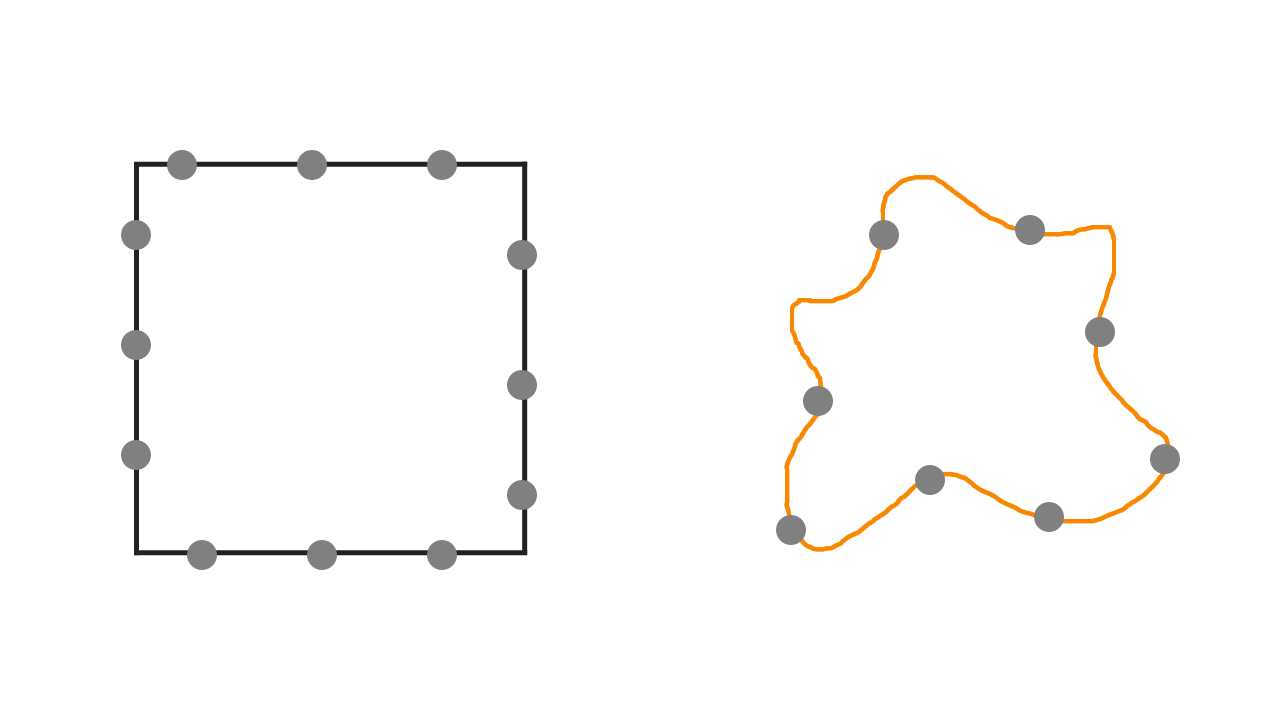
\includegraphics[width=0.3\paperwidth]{img/soil-systematic-sampling.png}
    \caption{Posible muestreo sistemático de un lote}
\end{figure}

La ilustración de arriba describe una de muchas estrategias \cite{lassaga-2011} \cite{gobpe-ministerio-del-ambiente-2014} para tomar las muestras del suelo. En este caso se toma el perímetro del suelo y sistemáticamente se toman las muestras por el perímetro, las cuales también pueden ser determinadas por otros patrones como diagonal o zigzag.

\bigbreak

Hay que tomar en cuenta que el muestreo sistemático no siempre produce una muestra representativa por lo dicho más arriba, esto es, cuando hay una distribución periódica de las unidades. Para los estudios ecológicos de suelos \cite{lohr-2009}: \say{Puede haber una topografía de crestas y surcos que daría lugar a un patrón periódico de vegetación. Si un esquema de muestreo sistemático sigue el mismo ciclo, la muestra no se comportará como una MAS}.

\section{Muestreo estratificado}

Como se ha mencionado, este es uno de los temas centrales de esta investigación ya que los suelos agrícolas se pueden \textit{particionar} en lotes los cuales tienen atributos que permiten su medición y se espera poder llegar a establecerlos como homogéneos para poder elaborar el diseño del muestreo correspondiente.

\bigbreak

La población se debe de dividir (particionar) en \textbf{estratos} que sean disjuntos a dos. Esto viene de la clásica estratificación por capas. Así, para una población de tamaño $N$, se divide en $H$ estratos o capas con $N_h$ unidades en el estrato $H$. Es necesario conocer $N_1$, $N_2$, ... , $N_H$ y por tanto se tiene que $N_1 + N_2 + \cdot \cdot \cdot + N_H = N$.

\bigbreak

Para hacer un \textbf{muestreo estratificado aleatorio} como es de esperar, se toma cada estrato de $N_h$ unidades y se hacen $n_h$ mediciones aleatorias ($n_h < N_h$). Entonces el tamaño de la población se encuentra dado por $n = \sum_{i=1}^H n_i$.

\bigbreak

Según la \textit{Guía de muestreo de suelo $\|$ Gob.Pe} \cite{gobpe-ministerio-del-ambiente-2014}, el muestreo aleatorio estratificado se hace \say{cuando se dispone de información previa y el sitio presenta 
características geográficas diferenciadas, es necesario estratificar o subdividir en subgrupos las 
muestras que tienen homogeneidad en el terreno y en cada estrato se aplica un muestreo 
aleatorio simple de manera independiente}.

\begin{figure}[H]
    \centering
    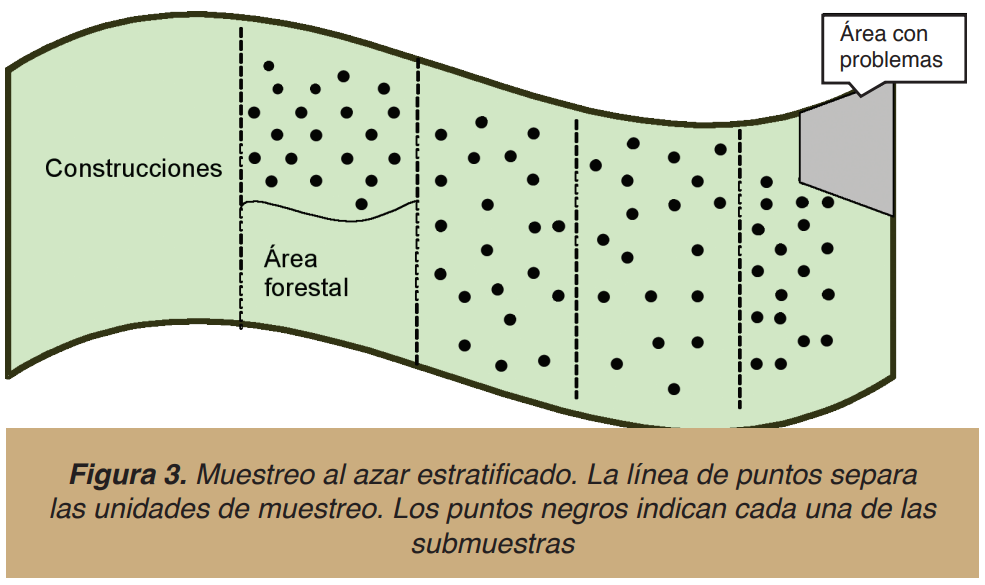
\includegraphics[width=0.5\paperwidth]{ref/stratified-sampling-examples.png}
    \caption{Ejemplo de estratos para diagnóstico de fertilidad \cite{lassaga-2011}}
\end{figure}

Como resumen de los tipos de muestreos de utilidad se puede ilustrar el siguiente ejemplo:

\begin{figure}[H]
    \centering
    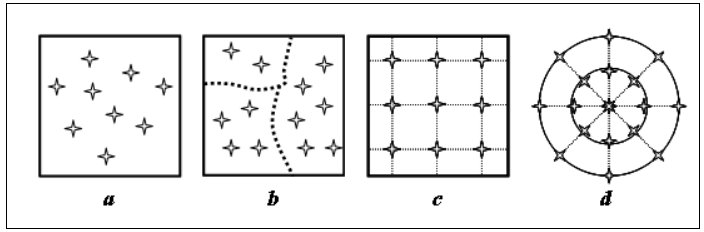
\includegraphics[width=0.5\paperwidth]{ref/kind-of-samplings-example.png}
    \caption{Ejemplo de tipos de muestreos. a) aleatorio simple, b) aleatorio estratificado, c) sistemático rejilla rectangular, d) sistemático rejilla polar \cite{innec-2007}}
\end{figure}

Sea $S_h$ el conjunto de $n_h$ unidades para el estrato $h$. El valor de la unidad \textit{jth} en el estrato $h$ se define como $x_{hj}$. Se siguen las siguientes valoraciones para el muestreo estratificado \cite{lohr-2009}:

\bigbreak

\textbf{Población total en el estrato H}
\bigbreak
$t_h = \sum_{j=1}^{N_h} x_{hj}$


\bigbreak

\textbf{Total de la población}
\bigbreak
$t = \sum_{h=1}^H t_h$


\bigbreak

\textbf{Media de la población para el estrato $h$}
\bigbreak
$\overline{x}_{hU} = \frac{\sum_{j=1}^{N_h} x_{hj}}{N_h} = \frac{t_h}{N_h}$


\bigbreak

\textbf{Media de la población en general}
\bigbreak
$\overline{x}_U = \frac{\sum_{h=1}^H \sum_{j=1}^{N_h} x_{hj}}{N} = \frac{t}{N}$


\bigbreak

\textbf{Varianza de la población en el estrato $h$}
\bigbreak
$S_h^2 = \sum_{j=1}^{N_h} \frac{(x_{hj} - \overline{x}_{hU})^2}{N_h - 1}$


\bigbreak

A partir de aquí, otros cálculos para los MAS se pueden aplicar para cada estrato. Se tiene que:

\bigbreak

$\overline{x}_h = \frac{1}{n_h} \sum_{j \in S_h} x_{hj}$

\bigbreak

$s^2_h = \sum_{j \in S_h} \frac{(x_{hj} - \overline{x}_h)^2}{n_h - 1}$

\bigbreak

El muestreo estratificado sin reemplazo basado en el MAS es el objetivo principal para obtener resultados bajo este marco teórico.

\subsection{Varianza}

Asumiendo que se tiene un muestreo estratificado donde cada estrato es relativamente homogéneo, la varianza de cada estrato es pequeña por lo que la varianza del estimado final también será pequeña, por consiguiente se sigue que \cite{gulland-1966}:

\bigbreak

Tenemos siempre que $N$ es el total de la población, $N_h$ es el $h$-ésimo estrato y $N=SN_h$. Una muestra de $n_h$ es tomada entonces del $h$-ésimo estrato, los valores que se desean estimar (longitud, peso, etc.) son dados por $x_{hj}$, $j=1,...,n_h$. De arriba, tenemos que la media estimada para el estrato $h$ es

$$
\overline{x}_h = \frac{1}{n_h} \sum_{h=1}^{n_h} x_{hj}
$$

Un estimado sin sesgo de la media en toda la población es dado por esta media ponderada:

$$
\overline{x} = \frac{1}{N} \sum_{h} N_h \overline{x}_h
$$

Si la varianza dentro del $h$-ésimo estrato es $S_h^2$

$$
var(\overline{x}_h) = \frac{1}{n_h} S_h^2
$$

y

$$
var(\overline{x}) = \frac{1}{N^2} \sum \frac{N_h^2}{n_h}S_h^2
$$

dado que $n_h$ sea pequeño comparado a $N_h$. Sino, las varianzas son dadas por

$$
var(\overline{x}_h = \frac{1}{n_h}(1 - \frac{n_h}{N_h})S_h^2
$$


$$
var(\overline{x}) = \frac{1}{N^2} \sum_h N_h^2 \frac{1}{n_h}(1 - \frac{n_h}{N_h})s_h^2 = \frac{1}{N^2} \sum_h N_h (N_h - n_h) \frac{1}{n_h} S_h^2
$$

Esta varianza puede ser comparada con la varianza del estimado obtenido al hacer el muestreo aleatorio de la población total:

$$
var(\overline{x}') = \frac{1}{n}S^2
$$

o

$$
var(\overline{x}) = \frac{1}{n}(1 - \frac{n}{N})S^2
$$

si $n$ no es pequeño comparado con $N$ donde $S^2$ es la varianza de la población total.

\subsection{Ejemplo}

En esta subsección se presenta un ejemplo con datos reales obtenido del \textit{Manual of Sampling and Statistical Methods for Fisheries Biology} \cite{gulland-1966}:

\bigbreak

\subsubsection{Barco de pesca comercial}

La captura de un arrastrero comercial que desembarca eglefino en Aberdeen \footnote{Aberdeen es una ciudad en Escocia \cite{wikipedia-aberdeen-2021}.} se clasificó en cuatro categorías de tamaño que forman los cuatro estratos. Se midieron muestras de eglefino \footnote{El eglefino es un miembro de la familia del bacalao con un sabor suave, carne firme y textura húmeda. Se usa indistintamente con el bacalao pero tiene un sabor ligeramente más dulce, lo que lo convierte en el mejor pescado blanco para ahumar. El eglefino se vende comúnmente fresco, congelado o ahumado \cite{sustainable-fishing-msc-marine-stewardship-council-2021}.} de cada categoría y los datos resultantes se pueden resumir de la siguiente manera:

\bigbreak

% ----- TABLE

\begin{table}[H]
\centering
\begin{tabular}{|l|l|l|l|l|}
\hline
\rowcolor[HTML]{CBCEFB} 
\multicolumn{1}{|c|}{\cellcolor[HTML]{CBCEFB}\textbf{Categoría}} & \multicolumn{1}{c|}{\cellcolor[HTML]{CBCEFB}\textbf{$N_h$}} & \multicolumn{1}{c|}{\cellcolor[HTML]{CBCEFB}\textbf{$n_h$}} & \multicolumn{1}{c|}{\cellcolor[HTML]{CBCEFB}\textbf{$Sx_{hj}$}} & \multicolumn{1}{c|}{\cellcolor[HTML]{CBCEFB}\textbf{$Sx_{hj}^2$}} \\ \hline
Pequeña                                                          & 2432                                                        & 152                                                         & 5284                                                            & 185532                                                            \\ \hline
\rowcolor[HTML]{EFEFEF} 
Pequeña-media                                                    & 1656                                                        & 92                                                          & 3817                                                            & 158953                                                            \\ \hline
Media                                                            & 2268                                                        & 63                                                          & 3033                                                            & 146357                                                            \\ \hline
\rowcolor[HTML]{EFEFEF} 
Grande                                                           & 665                                                         & 35                                                          & 2027                                                            & 118169                                                            \\ \hline
\rowcolor[HTML]{FFCE93} 
Total                                                            & 7021                                                        & 342                                                         & 14161                                                           & 609011                                                            \\ \hline
\end{tabular}
\caption{Datos para cada estrato de la captura del barco de pesca}
\end{table}

% ----- END TABLE

donde $x$ es la longitud del pescado en $cm$.

Entonces usando como estimado de $S_h^2$ la ecuación:

$$
S_h^2 = \frac{1}{n_h - 1} \left[ \sum_{h=1}^{N_h} x_{hj}^2 - \frac{1}{n_h} \left(\sum_{h=1}^{N_h}x_{xj} \right)^2 \right]
$$

también tenemos que:

% ----- TABLE

\begin{table}[H]
\centering
\begin{tabular}{|l|l|l|l|l|l|}
\hline
\rowcolor[HTML]{CBCEFB} 
\multicolumn{1}{|c|}{\cellcolor[HTML]{CBCEFB}\textbf{Categoría}} & \multicolumn{1}{c|}{\cellcolor[HTML]{CBCEFB}\textbf{$x_h$}} & \multicolumn{1}{c|}{\cellcolor[HTML]{CBCEFB}\textbf{$N_hx_h$}} & \multicolumn{1}{c|}{\cellcolor[HTML]{CBCEFB}\textbf{$S_{h}^2$}} & \multicolumn{1}{c|}{\cellcolor[HTML]{CBCEFB}\textbf{$\frac{S_{h}^2}{n_h}$}} & \textbf{$\frac{N_h^2S_h^2}{n_h}$} \\ \hline
Pequeña                                                          & 34.763                                                      & 84,544                                                         & 12.21                                                           & 0.0803                                                                      & 474,900                           \\ \hline
\rowcolor[HTML]{EFEFEF} 
Pequeña-media                                                    & 41.489                                                      & 68,706                                                         & 6.47                                                            & 0.0703                                                                      & 192,800                           \\ \hline
Media                                                            & 48.143                                                      & 109,188                                                        & 5.48                                                            & 0.0870                                                                      & 447,500                           \\ \hline
\rowcolor[HTML]{EFEFEF} 
Grande                                                           & 57.914                                                      & 38,513                                                         & 22.85                                                           & 0.6529                                                                      & 288,700                           \\ \hline
\rowcolor[HTML]{FFCE93} 
Total                                                            &                                                             & 300,951                                                        &                                                                 &                                                                             & 1,403,900                         \\ \hline
\end{tabular}
\end{table}

% ----- END TABLE

Así:

\bigbreak

$\overline{x} = \frac{300,951}{7,021} = 42.9$

\bigbreak

$var(\overline{x}) = \frac{300,951}{(7,021)^2} = 0.0285$

\bigbreak

$s.d(\overline{x}) = 0.17$

\bigbreak

El $95\%$ de confianza para la longitud media real del pescado establece dicho intervalo en $42.9 \pm (2 \cdot 0.17)$ esto es, $42.6-43.2 \, cm$.

\section{Patrones de muestreo}

Un patrón de muestreo se puede aplicar por ejemplo, a cada estrato de un muestreo estratificado. En el caso más trivial se puede hacer referencia a un patrón aleatorio, en otros casos se puede utilizar uno más elaborado. Esta sección recopila los patrones de muestreos de acuerdo a la \textit{Guía de muestreo de suelo $\|$ Gob.Pe} \cite{gobpe-ministerio-del-ambiente-2014}.

\bigbreak

Los patrones de muestreo se clasifican de acuerdo a si son: con distribución uniforme, con distribución aleatoria y con distribución heterogénea.

\subsection{Con distribución aleatoria}

Estos patrones de muestreo son utilizados en estadística.

\bigbreak

\textbf{Aleatorio:} Los puntos se escogen de forma aleatoria. Los resultados son muy irregulares.

\bigbreak

\textbf{Aleatorio sobre rejilla regular (estratificado):} El plano se divide (particiona) en zonas (estratos), se delimita un grid regular en todo el plano y se escoge un número igual de puntos distribuidos aleatoriamente en cada celda. Ya se ha hablado a más detalle de este patrón en secciones anteriores. La desventaja es que la forma en que están distribuidos los puntos puede ser muy dispersa, estando unos muy cerca y otros muy lejos por lo que quedan brechas de espacio vacío a menudo.

\bigbreak

\textbf{Aleatorio desalineado sobre rejilla regular:} Es una variante del patrón estratificado. En algunas celdas, la coordenada "x" se mueve al azar y en el resto de las celdas se mueve la coordenada "y", o viceversa. La desventaja también se hereda del método estratificado.

\begin{figure}[H]
    \centering
    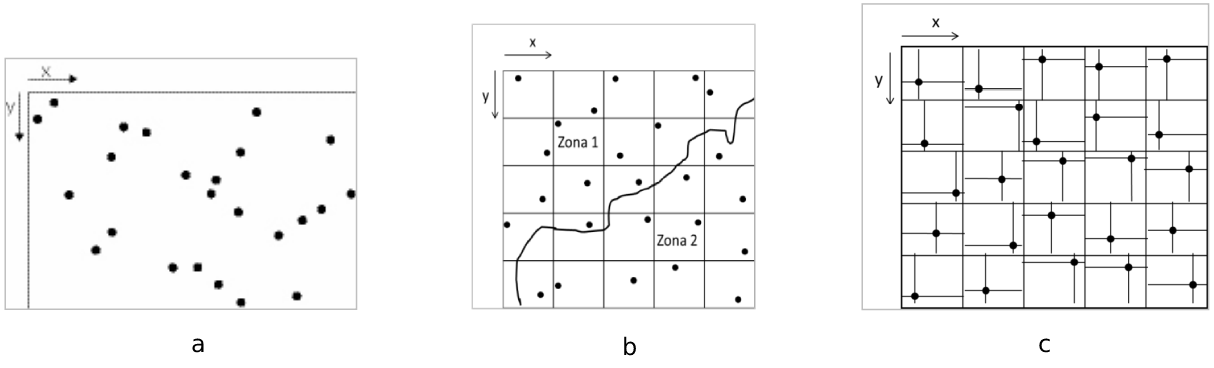
\includegraphics[width=0.7\paperwidth]{ref/random-sampling-patterns.png}
    \caption{Patrones de muestreo con distribución aleatoria}
    a) Aleatorio, b) Aleatorio sobre rejilla regular, c) Aleatorio desalineado sobre rejilla regular \\
    Fuente: \textit{Guía de muestreo de suelo $\|$ Gob.Pe} \cite{gobpe-ministerio-del-ambiente-2014}
\end{figure}

\subsection{Con distribución uniforme}

\textbf{Rejillas regulares:} Se hace un grid de cuadrados en el plano donde cada celda es tan grande como se necesite (inversamente proporcionalmente al nivel de detalle). Por último se escoge el punto en cualquier parte de \textit{cada} celda verificando que la posición del punto sea la misma en todas las celdas.

\bigbreak

\textbf{Rejillas triangulares:} Se trazan triángulos equiláteros en el plano y se aplica el nivel de detalle establecido arriba.

\bigbreak

\textbf{Rejilla circular:} Para análisis de contaminación es de utilidad para delimitar la zona contaminada. Se trazan círculos concéntricos, separados de acuerdo al detalle requerido. Se trazan líneas rectas considerando los 8 puntos cardinales principales y se ubican los puntos de muestreo en las intersecciones. Se espera que con esta rejilla las mayores concentraciones de contaminantes se ubiquen en el centro.

\bigbreak

\textbf{Sobre una línea:} Este patrón también sirve para contaminantes cuando la contaminación siga una línea recta.

\bigbreak

\textbf{Diagonales múltiples:} Por último, con este patrón se traza una diagonal central y líneas paralelas en el plano, sobre las cuales se ubican los puntos de muestreo, manteniendo la misma distancia entre ellos.

\begin{figure}[H]
    \centering
    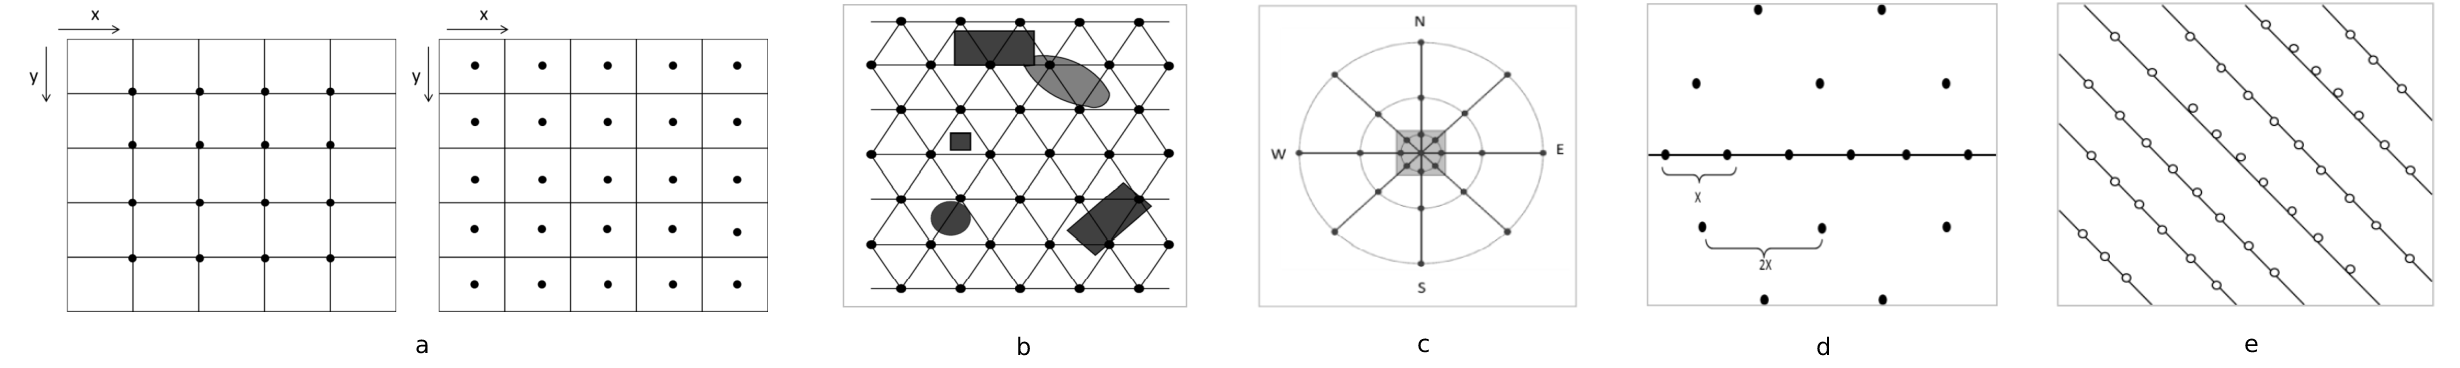
\includegraphics[width=0.7\paperwidth]{ref/uniform-sampling-patterns.png}
    \caption{Patrones de muestreo con distribución uniforme}
    a) Rejillas regulares, b) Rejillas triangulares, c) Rejilla circular, d) Sobre una línea, e) Diagonales múltiples \\
    Fuente: \textit{Guía de muestreo de suelo $\|$ Gob.Pe} \cite{gobpe-ministerio-del-ambiente-2014}
\end{figure}


\subsection{Con distribución heterogénea}

Por último se enumeran este otro tipo de patrones que se pueden encontrar en un muestreo físico. Estos consisten en:

\begin{itemize}
    \item Diagonal simple
    \item Diagonales cruzadas rotantes
    \item Muestreo irregular en forma de N, S, X, o W
    \item Zig-zag
    \item Zig-zag transverso
\end{itemize}

\section{Muestreo virtual}

En esta sección se documenta las diferentes salidas computacionales que son de gran importancia para trabajar con muestras de datos. Actualmente, el lenguaje de programación adoptado por la comunidad de científicos de datos y otras comunidades similares es Python debido a la estandarización que tienen sus librerías de matemáticas y ciencia de datos, además de la simplicidad de su sintaxis lo cual permite la creación de prototipos y de documentos interactivos con herramientas como Jupyter Notebook \footnote{Jupyter Notebook es una aplicación web de código abierto que permite crear y compartir documentos que contienen código en tiempo real, ecuaciones, visualizaciones y texto narrativo. Los usos incluyen: limpieza y transformación de datos, simulación numérica, modelado estadístico, visualización de datos, aprendizaje automático y mucho más \cite{jupyter-2021}.}. Toda la gama de bibliotecas y herramientas para matemática y análisis de datos es dada en su mayoría bajo licencias de código abierto permisivas (comúnmente BSD-3-Clause). La ventaja de Python es que como ya se mencionó, ha sido altamente adoptado por la comunidad por su facilidad de entrada para no-programadores y también a destacar que es un lenguaje de scripting \footnote{Un lenguaje de scripting es un lenguaje de programación para un entorno de ejecución (runtime) que automatiza la ejecución de tareas que, de otro modo, serían realizadas individualmente por un operador humano.} por lo que su función principal es servir de interfase (wrapper) para lenguajes de programación que suelen ser robustos, eficientes y \textit{sin abstracciones innecesarias} como C y Rust \footnote{La tendencia actual para modelos reales (no-prototipos) está empezando a emplear Rust en lugar de lenguajes similares como C y C++ y de lenguajes de entrada como Python, mostrado también por la revista Nature en \say{Why scientists are turning to Rust} \cite{nature-editorial-2020}.}.

\subsection{Enlaces}

Se enlistan las fuentes de los proyectos de relevancia que se necesitan para esta sección:

\begin{itemize}
    \item Python: \url{https://www.python.org}.
    \item Pandas: \url{https://pandas.pydata.org}.
    \item Matplotlib: \url{https://matplotlib.org}.
    \item GeoPandas: \url{https://geopandas.org}.
    \item NumPy: \url{https://numpy.org}.
    \item Plotly: \url{https://plotly.com}.
    \item Jupyter: \url{https://jupyter.org}.
    \item SciPy: \url{https://scipy.org}.
    \item StatsModels: \url{https://www.statsmodels.org}.
\end{itemize}

\subsection{Visualización de datos}

La visualización de datos es fundamental en la ciencia de datos de forma que se puede tener mucha información de forma compacta y estudiar los resultados al mismo tiempo.

\bigbreak

Los dos usos principales de la visualización de datos son \cite{grus-2015}:

\begin{itemize}
    \item Explorar datos.
    \item Comunicar datos.
\end{itemize}

La biblioteca matplotlib es sugerida \cite{grus-2015} para la visualización de datos simples que no requieran un entorno web. Las posibilidades son: gráficos de barra simples, gráficos de líneas y gráficos de dispersión.

\bigbreak

Otras bibliotecas de interés comprenden \textbf{seaborn} derivado de matplotlib para visualizaciones más complejas y bonitas, \textbf{D3.js} para visualizaciones sostificadas e interactivas para la web, \textbf{Bokeh} para visualizaciones $3D$ en Python y \textbf{ggplot} el cual es un port de la biblioteca ggplot2 de R. 

\subsection{Estadística}

Las bibliotecas de SciPy, pandas y StatsModels tienen una gran gama de funciones para aplicaciones de estadística. Por el resto, Python trae muchas construcciones para el manejo de funciones, vectores, operaciones y matrices aunque las matrices no son lo más fuerte de Python.

\subsection{GIS en la agricultura}

Con respecto a la visualización de los datos, se tiene en consideración que el sector agrícola cuenta o debería contar con el uso de GISs. Un \textbf{GIS (Geographic Information System)} es una herramienta que crea representaciones visuales de los datos y realiza análisis espaciales a fin de tomar decisiones informadas; combina hardware, software y datos \cite{hammonds-2019}.

\bigbreak

En agricultura, un GIS puede dar información sobre el suelo, en tanto a cómo está estructurado, las propiedades y condiciones que presenta. Esto también es muy útil para visualizar un muestreo de puntos en un mapa en $2D$. Los archivos con los que se suele trabajar estos gráficos son archivos shapefile.

\bigbreak

\textbf{Shapefile:} \say{Formato de datos utilizado por la mayoría de software GIS/FMIS para almacenar datos espaciales (por ejemplo, límites de campo, ubicaciones de puntos o los polígonos que representan celdas de la cuadrícula). Un shapefile se almacena como una colección de archivos con un nombre común pero con diferentes extensiones de archivo (por ejemplo, .shp, .shx y .dbf).} Fuente: NC State Extension \cite{nc-state-extension-2021}.

\bigbreak

La biblioteca GeoPandas es una buena opción para manipular archivos shapefile y otros gráficos vectoriales.

\section{Encuestas agrícolas}

A fin de obtener información precisa para poder diseñar un muestreo representativo y eficiente puede ser necesario hacer un análisis mediante encuestas y poder obtener uno de los modelos de muestreo que se conocen.

\bigbreak

Las encuestas agrícolas son muy complicadas y tienen un gran número de variables las cuales pueden comprender en tanto de \cite{organizacion-de-las-naciones-unidas-para-la-agricultura-y-la-alimentacion-1990}:

\begin{itemize}
    \item Herramientas, maquinarias, fertilizantes, plaguicidas, semillas y otros insumos.
    \item Superficie total y régimen de tenencia.
    \item Superficie bajo cultivos y producción.
    \item Verduras, frutas, nueces.
    \item Ganadería, avicultura, estabulación.
    
    \item Pesca, caza y explotación maderera.
    \item Regadío, pozos, avenamiento y cercado.
    \item Ingresos, comercialización, gastos, ahorros.
    \item Recuento y características de la población; mano de obra no pagada.
    \item Sanidad, educación, ocupación y estadísticas sociales de la población agrícola.
    \item Hogares y edificios agrícolas.
    \item Transporte y comunicaciones de la población agrícola.
    \item Fuentes y consumo de alimentos.
    \item Encuestas de opinión acerca de las políticas, métodos, productos, etc.
\end{itemize}

\bigbreak
    
Además de utilizar estas variables, se puede obtener más datos a partir de variables auxiliares. Con respecto a las fuentes de datos se puede acceder a los productores y las operaciones agrícolas, hogares agrícolas en relación con otros datos.

\bigbreak

Las encuestas agrícolas suelen ser muy variadas, cada variable que se ha enumerado tiene sus propias variaciones y propósitos múltiples. Por esto observamos que se deberá recurrir a \textbf{encuestas multitemáticas}. Además, también se necesitan aplicar métodos múltiples ya que las mediciones que se hacen requieren métodos diferentes de medición.

\section{Muestreo físico}

El muestreo que se suele realizar en agricultura es probablemente para los fines de análisis de fertilidad \cite{lassaga-2011} y de contaminación \cite{gobpe-ministerio-del-ambiente-2014}. Un procedimiento estándar de acuerdo a profesionales consiste de forma básica en utilizar equipo dedicado \cite{ministry-of-agriculture-food-and-fisheries-2020} o no, dependiendo si se necesitan hacer muchos muestreos o solo es una práctica amateur. Se toman unas $6 \, pulgadas$ de tierra y se recolectan en una cubeta. Este procedimiento se ha de repetir unas $10$ a $15$ veces para que la muestra sea más uniforme a fin de obtener la muestra a partir de las múltiples submuestras mencionadas. Luego se debe de mezclar la tierra de todas las submuestras. Finalmente, se toma la cantidad de muestra especificada por el laboratorio (una bolsa) de la tierra de la cubeta ya mezclada. Se deben llenar los datos y la muestra obtenida se envía para hacer el estudio. Uno de estos datos es especificar la muestra que se manda ya que pueden haber muchas muestras que se requieren diferenciar. El procedimiento se encuentra mejor documentado en el \textit{Noble Research Institute} \cite{funderburg-2014}.

\bigbreak

Para el muestreo del diagnóstico de fertilidad se diseña una estrategia con el siguiente estilo \cite{lassaga-2011}:

\begin{itemize}
    \item Delimitar el terreno en áreas homogéneas llamadas \textbf{unidades de muestreo}. Para esto se consideran los atributos de características físicas, topográficas y similares.
    
    \item Contar con un plano donde se vea como se dividió el terreno y con información geográfica relevante.
    
    \item Otras consideraciones.
\end{itemize}

Otros registros importantes en este puto son, a saber \cite{lassaga-2011}, el \textit{rendimiento} de los cultivos por áreas homogéneas e historiales con datos anteriores.

\bigbreak

A partir de aquí, muchas estrategias de muestreo, donde ya se han mencionado algunas, se pueden aplicar para llevar a cabo este trabajo de muestreo convencional de suelo.

\subsection{Tipos de errores}

Hay varios tipos de errores al tomar muestras. Adelante se muestran algunas más comunes \cite{innec-2007}. Los errores por tener un muestreo sesgado conllevan hasta pérdidas multi-billionarias \cite{gy-1998}. El siguiente caso sucedido hace ya muchas décadas es sobre una mina que fue (Pierre, 1998):

\bigbreak

\say{En un caso legal entre una mina de estaño y una fundición, se demostró que el muestreo sesgado en la fundición había infravalorado los concentrados de la mina, durante un período de varios años, en un factor de $9\%$. ¿Qué industria permitiría a sabiendas que se se va a descontar el $9\%$ del valor de sus producciones? ¿Existe alguna otra operación capaz de provocar una pérdida? ¡Nunca!}

\bigbreak

Así también hay muchos otros casos donde los errores en los muestreos han sido muy costosos. La ventaja de hoy en día es que se cuenta con mucha tecnología a diferencia de esa época.

\bigbreak

% ----- TABLE
\begin{table}[H]
\centering
\begin{tabular}{|l|l|l|}
\hline
\rowcolor[HTML]{CBCEFB} 
\multicolumn{1}{|c|}{\cellcolor[HTML]{CBCEFB}\textbf{Tipo de error}}       & \multicolumn{1}{c|}{\cellcolor[HTML]{CBCEFB}\textbf{Causa}}                                                                                 & \multicolumn{1}{c|}{\cellcolor[HTML]{CBCEFB}\textbf{Forma de minimización}}                                                               \\ \hline
Fundamental                                                                & \begin{tabular}[c]{@{}l@{}}Pérdida de precisión en la muestra, \\ debido a su composición física y \\ química\end{tabular}                  & \begin{tabular}[c]{@{}l@{}}Disminución del diámetro de las partículas\\  más grandes o aumento de la masa de la\\  muestra\end{tabular}   \\ \hline
\rowcolor[HTML]{EFEFEF} 
\begin{tabular}[c]{@{}l@{}}Segregación \\ y agrupación\end{tabular}        & \begin{tabular}[c]{@{}l@{}}Se debe a la distribución no al azar \\ de partículas, usualmente por efecto \\ de la gravedad\end{tabular}      & \begin{tabular}[c]{@{}l@{}}Preparación al azar de muestras compuestas\\ u homogeneización y fraccionamiento de\\  la muestra\end{tabular} \\ \hline
\begin{tabular}[c]{@{}l@{}}Heterogeneidad\\  de largo alcance\end{tabular} & Error espacial y fluctuante y no a alzar                                                                                                    & \begin{tabular}[c]{@{}l@{}}Toma de muchos incrementos para formar \\ una muestra\end{tabular}                                             \\ \hline
\rowcolor[HTML]{EFEFEF} 
\begin{tabular}[c]{@{}l@{}}Heterogeneidad\\  periódica\end{tabular}        & Error de fluctuación temporal o espacial                                                                                                    & \begin{tabular}[c]{@{}l@{}}Generación correcta de muestras \\ compuestas\end{tabular}                                                     \\ \hline
\begin{tabular}[c]{@{}l@{}}Delimitación de \\ incrementos\end{tabular}     & \begin{tabular}[c]{@{}l@{}}Diseño de muestreo inapropiado y/o\\  mala selección de equipo\end{tabular}                                      & \begin{tabular}[c]{@{}l@{}}Diseño del muestreo y selección \\ apropiada de equipo\end{tabular}                                            \\ \hline
\rowcolor[HTML]{EFEFEF} 
\begin{tabular}[c]{@{}l@{}}Extracción de\\  incrementos\end{tabular}       & \begin{tabular}[c]{@{}l@{}}El procedimiento de muestreo falla \\ en cuanto a la extracción precisa del\\  incremento propuesto\end{tabular} & \begin{tabular}[c]{@{}l@{}}Indispensable contar con los protocolos\\ adecuados y equipo de muestreo bien \\ diseñado\end{tabular}         \\ \hline
Preparación                                                                & \begin{tabular}[c]{@{}l@{}}Se debe a pérdidas, contaminación \\ y/o alteración de una muestra\end{tabular}                                  & \begin{tabular}[c]{@{}l@{}}Existen técnicas de campo y laboratorio\\ para evitar el problema\end{tabular}                                 \\ \hline
\end{tabular}
\caption{Tipos de errores de muestreo y técnicas para su minimización}
Fuente: Gobierno de México $\|$ Instituto Nacional de Ecología y Cambio Climático \cite{innec-2007}
\end{table}
% ----- END TABLE

Muchas de estas soluciones para este tipo común de errores deben de ayudar a mejorar las técnicas de muestreo. Definitivamente es recomendable que el usuario que realiza la muestra física sea asesorado con estas guías las cuales se extienden mucho más allá de este estudio y son fundamentales para salvar enormes cantidades económicas y tener una ciencia de datos más correcta.

\chapter{Anexos}

Se ha tomado nota en pequeña parte sobre la elaboración y estructura de \textit{Manual de Elaboración y Presentación de Tesis} \cite{universidad-san-carlos-2016}, \textit{Metodología de la investigación} \cite{collado-2014}, \textit{Introducción a la metodología de la investigación científica} \cite{cabezas-2018} para esta propuesta de investigación.

\section{Glosario}

\begin{itemize}
    \item \textbf{Analítica:} Proceso de detectar, interpretar y comunicar patrones significativos en los datos, así como usar herramientas para que toda la organización pueda realizar cualquier pregunta sobre cualquier información en todos los entornos y dispositivos posibles \cite{oracle-2021}.
    
    \item \textbf{Rendimiento:} Razón con unidad dimensional [MASA][PRODUCTO]/[ÁREA] útil para medir el beneficio producido en una zafra (p. ej. 1TA/HA 1 tonelada de azucar por hectárea).
    
    \item \textbf{Zafra:} Cosecha de la caña dulce (p. ej. zafra 2020-2021).
\end{itemize}

\subsubsection{Términos de dominio específico}

\begin{itemize}
    \item \textbf{Usuario:} Empresa agrícola en Honduras.
    
    \item \textbf{Usuario interno:} Empleado de la empresa agrícola.
    
    \item \textbf{Muestreo físico:} Muestra original que el usuario tomó en su suelo agrícola.
    
    \item \textbf{Muestreo virtual:} Resultado o salida del modelo que se ha de desarrollar en este estudio el cual tiene como entrada el muestreo físico.
    
    \item \textbf{Curar:} Transformar los datos originales mediante filtros de forma que se eliminen los todos aquellos datos innecesarios o corruptos para el análisis subyacente.
\end{itemize}

\printbibliography

\end{document}
